\documentclass[11pt,twocolumn]{ctexart}

\usepackage{multicol}
%\usepackage{mwe}
\usepackage{subfigure}
\usepackage{mathtools}
\usepackage{graphicx}
\usepackage{amsmath}
\usepackage{mathrsfs}
\usepackage[top=0.5in,bottom=1in,left=1in,right=1in]{geometry}
\usepackage{pdflscape}
\usepackage{times}
\usepackage{bm}
%\usepackage{setspace}
\usepackage{color}
\usepackage{caption}
\usepackage{amsmath}
\usepackage{amssymb}
%\usepackage{CJK}
%\usepackage[final]{pdfpages}
\usepackage{listings}
\usepackage{textcomp}
\usepackage{xcolor}
\pagestyle{plain}



\begin{document}

\title{利用简单的量子比特算法调和计算多极化世界文化强度和力量关系\\
\begin{large}
阅读文明的冲突与世界秩序的重建读书报告
\end{large}}
\author{北京大学光华管理学院20级袁俊一}
\date{\today}

\twocolumn[
    \begin{@twocolumnfalse}		
    \maketitle % need full-width title



   \begin{flushleft}
   \noindent        %段落的不缩进
   \hangafter=0     %从当前位置开始段落变窄
   \setlength{\hangindent}{2em} %变窄系数

   {{\textbf{摘要:} 量子计算机硬件的关键在于量子门操作。两个量子比特门是实现量子信息处理器的主要途径。在这里,我们提出了一个两量子比特门构成的可调耦合器,通过调制耦合器的频率来控制量子比特和量子比特的耦合。两个量子比特门的操作可以通过在色散区操作耦合器来实现,这对量子比特的状态是无影响的。我们模拟了一个通用的两量子比特耦合机制来研究该方案,最后得出了理想的效果。}}

   {{\textbf{关键词:} 相交理论;层论;Hodge理论;代数几何方法;代数流形方法;多极化世界;文化簇;文化极;社会关系;基本价值}}
   \vspace{0.2in}

   \end{flushleft}

    \end{@twocolumnfalse}
]



\CTEXsetup[format={\Large\bfseries}]{section}

\section{前言}
世界文明和文化存在两个世界,分别是西方世界和其他世界。西方世界文化存在中心论,亨廷顿对世界格局的研究存在去中心化,嘲讽和驳斥中心论,认为其中鲜有共同点和其他世界相关联。无论价值、思想、宗教的内容都没有相关联的部分。西方世界虽然通过其思想、价值或宗教的优越极力向外扩张和传输他们的价值观、思想和宗教,但是伴随着有组织的暴力和军事的优势进行扩张[1]。

亨廷顿认为,西方世界和西方文化通过西方世界的商品和武力而变得西方化,对此西方世界并不认为并且经常忽略,极其幼稚和妄自尊大。非西方文化和非西方世界对于惯常的西方中心论已经开始反弹,这意味着西方的扩张的终结,而对西方的反抗的开始了。

亨廷顿认为去西方世界的中流砥柱,来自西亚世界和西亚社会的自我认知。财富是道德和文化优越性的证明,亚洲财富的积累使得去西方化有厚实的基础,用西方的东方学曾用来描绘东方时所持的同样的否定态度来描绘西方,具有亚洲普世主义色彩。亨廷顿总结其遇到的三个问题:它是错误的,不道德的,以及危险的。而且更一针见血地指出,普世主义的必然逻辑结果是帝国主义。不过我其实觉得,现今人类的觉悟下,强者的文化=普世文化,进而蜕变为帝国主义,是无法避免的,不只是西方人自大而已。他说亚洲的时候不是顺理成章就想象了“亚洲普世主义”吗?中国现在不是被称作新帝国主义了吗?不过,新的东方帝国崛起来对抗一下旧的西方帝国,达成某种平衡,总好过一头独大就是了。

量子信息技术是量子物理与信息科学交叉的新生学科,其物理基础是量子力学。量子信息技术主要的应用领域包括量子计算、量子通信和量子测量等。进入21世纪之后,人类对微观粒子系统的观测和调控技术不断和提升,使得量子操作成为可能,量子信息技术蓬勃发展,已经成为物理和计算机学科的第一大热点,在2020年,开始兴起爆发的第二次量子科技革命,其主角就是以量子计算和量子们操作技术。量子科技在自然语言分析,机器学习技术,结构性理论的验证等很多方面起着举足轻重的作用。量子科技所解决的问题,可以覆盖几乎所有领域,拥有高度精确和绝对安全的黑箱属性。通过量子们解决问题,可以不关心问题的解决过程,利用量子技术和爱因斯坦方程调和解决问题。在(Li et al.2019)的文章中,利用量子门电路解决了单细胞生物的族群协同特性,模拟了线虫族群的集体表观形态和唯象理论的理论结果,取得了重大进展。在(zhang, Jun, et al. 2019)的文章中,利用量子门电路进行了多向性操作,证实了量子电路的全同性和统一性,为在其他很多学科的跨学科交叉应用提供了重要条件。在(Weirstreress, pock, et al.2020)的文章中,利用量子门电路模拟了简单粒子系统,是非常重要的结果。一般认为,粒子系统可以应用在很多方面,模拟生物学和生态学过程,模拟社会学进程,模拟艺术文化发展以及相应的定量计算和精确研究都非常有效,量子技术也顺理成章地可以应用在世界文化研究和世界格局系统上,进行研究和模拟其演化发展过程。我国在量子计算领域目前还是以研究为主,但是我国加大量子科技投入,而且各地方量子通信网络建设和各行业量子科技试点应用正在加速推进。我也希望能用所学知识和我做的研究方法,对亨廷顿所研究的世界模型进行建模,利用量子技术进行模拟和反演,得到一些先验性质的结论。

量子信息操作成为[2,3]处理器体系结构的最新发展一直集中在可扩展性[1-5]。高质量的门操作是这些中等规模量子处理器的关键性能指标之一[6]。由于门的性能最终决定了器件能否显示出量子优势,因此在这些系统中开发高质量的门成为当务之急。改进门特性显著降低了实现基于门的量子纠错码所需的开销,并提高了量子模拟的性能。今天量子门操作的主要限制因素是相对故障的两量子比特门。因此,提高双量子比特门特性是实现大规模量子处理器的当务之急。

一般来说,门误差有两个来源:去相干(随机)和非理想相互作用(确定性)。后者包括寄生耦合、对非计算状态的泄漏和控制串扰。作为寄生耦合的一个例子,次近邻(NNN)耦合是许多系统中常见的现象,包括里德堡原子[4,7]、俘获离子[5,8]、半导体自旋量子比特[9,10]和超导量子比特[11,12]。通常,NNN耦合被认为是非常重要的,并且在原本不相连的量子位之间引入了不必要的交互作用。

同时,可调耦合器可以帮助解决频率拥挤的问题,这种拥挤加剧了非理想相互作用的效果。可调谐耦合器的原型已经在超导量子电路中得到了广泛的证明[13-22]。然而,这些附加元素通常会增加体系结构的复杂性,并为消相干和串扰开辟了新的通道。其中,gmon设计[19]是一个成功的例子,它展示了一个主要由退相干控制的两个量子比特的栅极限制。然而,与前一代xmon设计相比,可调谐耦合器减少了gmon电路中量子比特的相干时间[11]。

在这项工作中,我们提出了一个简单而广泛应用的方案,用可调耦合器来实现高精度的两个量子比特门。该方法基于一个具有交换型交互作用的一般三体系统。一个核心部件,耦合器,频率调谐两个量子比特之间的虚拟交换交互作用,并具有一个临界偏压点,在该点上,交换相互作用将设置直接量子比特-量子比特(NNN)耦合,从而有效地转离网络耦合。两个量子比特门操作是通过在色散区操作耦合器来执行的,从而强烈地抑制了对耦合器激发态的泄漏。我们基于我们组[23]和其他[11]中现有的高相干超导量子硬件来模拟iSWAP门。我们发现,由于寄生效应引起的栅极误差随着栅极时间的增加(相互作用幅度的减小)急剧减小。在没有退相干的情况下,在100ns内可以实现99.999%以上的门特性。与高相干性体系结构的兼容性、对寄生效应的强烈抑制以及NNN耦合的利用,使我们的方案在相干时间不断提高的情况下成为长期可行的选择。


\section{模型}
\subsection{}
我们考虑一个由三个模式链组成的一般系统,最近邻和次近邻之间有交换耦合,如图1(a)所示。两个量子位(ω1和ω2)分别耦合到耦合强度为gj(j=1,2)的中心可调谐耦合器(ωc),以及耦合强度为g12的相互耦合。最近邻(NN)耦合一般强于NNN耦合,gj>g12>0。在不失一般性的前提下,我们从两能级哈密顿量开始分析,
哪里?(=1,2,c)分别是对应模式的本征基中定义的pauli Z,升高和降低算子。我们假设两个量子比特都与耦合器负失谐,

这个系统的真实性。两个量子比特通过两个通道相互作用,直接的NNN耦合和通过耦合器的间接耦合。后者有时被称为虚拟交换交互[24],这可以被schrieffer-wolfff变换(SWT)U所近似

mation=将耦合器从系统中解耦到第二阶,单位为gj/,每种模式产生一个有效的2量子比特哈密顿量,

式中,ω?j=ωj+gj2/j是兰姆移位量子比特频率,$1/=(1/1+1/2)/2<0$。这里,我们还假设耦合器模式始终保持在基态。

\begin{equation}
\begin{split}
H =\sum_{j=1,2} \frac{1}{2} \omega_j \sigma_j^z + \frac{1}{2} \omega_c  \sigma_c^z +  \\ \sum_{j=1,2} g_j (\sigma_j^{+} \sigma_c^{-} + \sigma_j^{-} \sigma_c^{+}) +  \\ g_{12}(\sigma_1^{+}\sigma_2 ^{-} +\sigma_1^{+}\sigma_2^{-} + \sigma_1^{-}\sigma_2^{+})
\end{split}
\end{equation}

\begin{equation}
\begin{split}
\widetilde{H} = \sum_{j=1,2} \frac{1}{2} \widetilde{\omega_j} \sigma_j^z +[\frac{g_1 g_2}{\Delta} + g_{12}] \\ (\sigma_1^{+}\sigma_2 ^{-} +\sigma_1^{+}\sigma_2^{-} + \sigma_1^{-}\sigma_2^{+})
\end{split}
\end{equation}


\begin{figure}[h]
\begin{center}
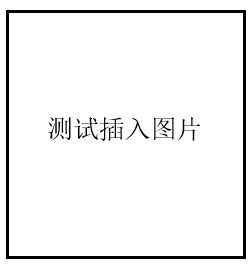
\includegraphics[width=0.4\textwidth]{fig1.png}
\end{center}
\caption{链几何中的一般三体系统的草图,其中中心模式是可调耦合器。}
\label{FIG.1}
\end{figure}

\begin{figure}[h]
\begin{center}
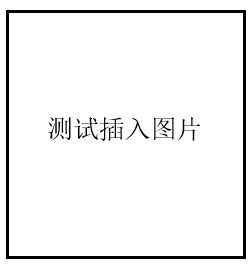
\includegraphics[width=0.3\textwidth]{fig2.png}
\end{center}
\caption{系统地和一个励磁状态的水平图。ket符号遵循链式顺序|ω1,ωc,ω2。往返箭头指示NN(橙色)和NNN(绿色)耦合。}
\label{FIG.2}
\end{figure}

\begin{figure}[h]
\begin{center}
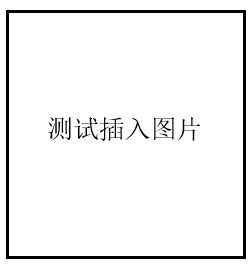
\includegraphics[width=0.5\textwidth]{fig3.png}
\end{center}
\caption{对(b)中的能级图进行schrieffer-wolfff变换后的两量子比特系统的能级图。每个图对应于有效负(左)、零(中心)和正(右)净耦合的情况,g∮。双头箭头表示耦合的符号和大小。在本例中,NNN耦合(绿色)为正且固定。NN耦合(橙色)是负的,可以用耦合器能量(实心黑线)调谐。}
\label{FIG.3}
\end{figure}



\subsection{第二章,第一节题目}
式(2)方括号内的组合项表示总有效量子位-量子位耦合g∮。它可以通过以及g1和g2通过耦合器频率进行调整,这两个参数都可能隐含地依赖于ωc。因此,g∮通常是ωc的函数。此外,由于<0,方括号中的第一项虚拟交换交互作用为负。这使得正直接耦合和负耦合之间的竞争成为可能间接耦合。如图1(c)所示,当耦合器频率降低时,可将g∮(ωc)调为负值,当耦合器频率增加时,可将g∮(ωc)调为正。最重要的是,由于可调性是连续的,因此只要耦合器的带宽允许,始终可以找到一个临界值ωcof,在该临界值下,这两个项可以消除,从而使耦合变差,即g∮(ωco off)=0。注意,色散极限条件只是一个理想的要求。在具有相当大的g12的系统中,仍然有可能在弱分散区(gj<|j |)中找到这样的ω系数[26]。

可调耦合器用于通过在空转期间将其频率偏置在ωcoff来消除相互作用。为了激活两个量子比特的相互作用,可以将耦合器频率调谐到所需的值ωcon,从而产生有限的g∮(ωcon)。该方案的特点有三个:(1)两个量子比特门可以通过只调制耦合器频率而不干扰量子比特来实现。(2) 通过在色散极限下操作耦合器,在SWT[等式(2)]之后被忽略的高阶项的寄生效应被强烈抑制,从而导致更高的两量子比特栅极特性。(3) 此外,该方案通过将其引入耦合器中,解决了不必要的NNN耦合问题。例如,如果两个量子位是共振的,则可以通过打开它们的耦合一定时间来实现iSWAP门。在此过程中,控制哈密顿量σcz在色散近似下与量子位的自由度进行换算,从而减少了对非定常(耦合器)状态的泄漏。这种情况下的非绝热效应被相对较大的量子比特耦合器失谐(j)所抑制,允许更短的栅极时间,从而减少退相干误差。


\section{结论}

最后,在这篇文章里,我们提出了一个简单而通用的可调耦合器方案。通过耦合器设置直接量子比特-量子比特耦合和虚拟交换交互,可以完全关闭耦合器,达到最后的目的。通过在色散区操作耦合器,可以有效地减少非理想情况对量子耦合门电路的门误差。因此,我们的方案在理论上是可行的,在实验上,具有一定的可实行性质,可以进行实验和操作来验证。同时,时间的一致性很难保证,还需要大量的实验和理论结论来进行进一步的改善。


\section{致谢}
感谢吴腾老师和郭宏老师这学期的付出和授课,感谢助教老师的辛勤付出和答疑,感谢学院量子材料中心的何琼毅老师给我的题材和内容,感谢对这门课有帮助的老师和同学,希望你们学习进步,工作顺利。


\begin{thebibliography}{1}
\bibitem{ref1} K.Jensen, V.M.Acosta, J.M.Higbie, et al. Cancellation of nonlinear Zeeman shifts with light shifts[J]. Physical Review A, 2009, 79(2):023406.

\bibitem{ref1} Chao Song, Kai Xu, Wuxin Liu, Chui-Ping Yang, Shi-Biao Zheng, Hui Deng, Qiwei Xie, Keqiang Huang, Qiujiang Guo, Libo Zhang, Pengfei Zhang, Da Xu, Dongning Zheng, Xiaobo Zhu, H. Wang, Y.-A. Chen, C.-Y. Lu, Siyuan Han, and Jian-Wei Pan, 10-Qubit Entanglement and Parallel Logic Operations with a Superconducting Circuit, Phys. Rev. Lett. 119, 180511 (2017).

\bibitem{ref1} Hannes Bernien, Sylvain Schwartz, Alexander Keesling, Harry Levine, Ahmed Omran, Hannes Pichler, Soon-won Choi, Alexander S. Zibrov, Manuel Endres, Markus Greiner, Vladan Vuletic, and Mikhail D. Lukin, Probing many-body dynamics on a 51-atom quantum simulator, Nature 551, 579 (2017).

\bibitem{ref1} J. Zhang, G. Pagano, P. W. Hess, A. Kyprianidis, P. Becker, H.Kaplan, A. V. Gorshkov, Z. X. Gong, and C. Mon-roe, Observation of a many-body dynamical phase transi-tion with a 53-qubit quantum simulator, Nature 551, 601 (2017).
\bibitem{ref1}John Preskill, Quantum computing in the nisq era and beyond, (2018).

\bibitem{ref1} M. Viteau, M. G. Bason, J. Radogostowicz, N. Mal-ossi, D. Ciampini, O. Morsch, and E. Arimondo, Rydberg Excitations in Bose-Einstein Condensates in Quasi-One-Dimensional Potentials and Optical Lattices, Phys. Rev. Lett. 107, 060402 (2011).

\bibitem{ref1} Joseph W. Britton, Brian C. Sawyer, Adam C. Keith, C.-C. Joseph Wang, James K. Freericks, Hermann Uys, Michael J. Biercuk, and John J. Bollinger, Engineered two-dimensional Ising interactions in a trapped-ion quantum simulator with hundreds of spins, Nature 484, 489 (2012).


\end{thebibliography}

\end{document} 